\documentclass[man,floatsintext]{apa6}
\usepackage{lmodern}
\usepackage{amssymb,amsmath}
\usepackage{ifxetex,ifluatex}
\usepackage{fixltx2e} % provides \textsubscript
\ifnum 0\ifxetex 1\fi\ifluatex 1\fi=0 % if pdftex
  \usepackage[T1]{fontenc}
  \usepackage[utf8]{inputenc}
\else % if luatex or xelatex
  \ifxetex
    \usepackage{mathspec}
  \else
    \usepackage{fontspec}
  \fi
  \defaultfontfeatures{Ligatures=TeX,Scale=MatchLowercase}
\fi
% use upquote if available, for straight quotes in verbatim environments
\IfFileExists{upquote.sty}{\usepackage{upquote}}{}
% use microtype if available
\IfFileExists{microtype.sty}{%
\usepackage{microtype}
\UseMicrotypeSet[protrusion]{basicmath} % disable protrusion for tt fonts
}{}
\usepackage{hyperref}
\hypersetup{unicode=true,
            pdftitle={Assessing sampling methods for generalization from RCTs: Modeling recruitment and participation},
            pdfauthor={Gleb Furman~\& James E. Pustejovsky},
            pdfkeywords={generalizability, sampling, MRT},
            pdfborder={0 0 0},
            breaklinks=true}
\urlstyle{same}  % don't use monospace font for urls
\usepackage{graphicx,grffile}
\makeatletter
\def\maxwidth{\ifdim\Gin@nat@width>\linewidth\linewidth\else\Gin@nat@width\fi}
\def\maxheight{\ifdim\Gin@nat@height>\textheight\textheight\else\Gin@nat@height\fi}
\makeatother
% Scale images if necessary, so that they will not overflow the page
% margins by default, and it is still possible to overwrite the defaults
% using explicit options in \includegraphics[width, height, ...]{}
\setkeys{Gin}{width=\maxwidth,height=\maxheight,keepaspectratio}
\IfFileExists{parskip.sty}{%
\usepackage{parskip}
}{% else
\setlength{\parindent}{0pt}
\setlength{\parskip}{6pt plus 2pt minus 1pt}
}
\setlength{\emergencystretch}{3em}  % prevent overfull lines
\providecommand{\tightlist}{%
  \setlength{\itemsep}{0pt}\setlength{\parskip}{0pt}}
\setcounter{secnumdepth}{0}
% Redefines (sub)paragraphs to behave more like sections
\ifx\paragraph\undefined\else
\let\oldparagraph\paragraph
\renewcommand{\paragraph}[1]{\oldparagraph{#1}\mbox{}}
\fi
\ifx\subparagraph\undefined\else
\let\oldsubparagraph\subparagraph
\renewcommand{\subparagraph}[1]{\oldsubparagraph{#1}\mbox{}}
\fi

%%% Use protect on footnotes to avoid problems with footnotes in titles
\let\rmarkdownfootnote\footnote%
\def\footnote{\protect\rmarkdownfootnote}


  \title{Assessing sampling methods for generalization from RCTs: Modeling recruitment and participation}
    \author{Gleb Furman\textsuperscript{1}~\& James E. Pustejovsky\textsuperscript{1}}
    \date{}
  
\shorttitle{Assessing sampling methods for generalization from RCTs}
\affiliation{
\vspace{0.5cm}
\textsuperscript{1} University of Texas at Austin}
\keywords{generalizability, sampling, MRT}
\usepackage{csquotes}
\usepackage{upgreek}
\captionsetup{font=singlespacing,justification=justified}

\usepackage{longtable}
\usepackage{lscape}
\usepackage{multirow}
\usepackage{tabularx}
\usepackage[flushleft]{threeparttable}
\usepackage{threeparttablex}

\newenvironment{lltable}{\begin{landscape}\begin{center}\begin{ThreePartTable}}{\end{ThreePartTable}\end{center}\end{landscape}}

\makeatletter
\newcommand\LastLTentrywidth{1em}
\newlength\longtablewidth
\setlength{\longtablewidth}{1in}
\newcommand{\getlongtablewidth}{\begingroup \ifcsname LT@\roman{LT@tables}\endcsname \global\longtablewidth=0pt \renewcommand{\LT@entry}[2]{\global\advance\longtablewidth by ##2\relax\gdef\LastLTentrywidth{##2}}\@nameuse{LT@\roman{LT@tables}} \fi \endgroup}
\usepackage{rotating}
\usepackage{float}

\authornote{

Correspondence concerning this article should be addressed to Gleb Furman, University of Texas at Austin, SZB 504, 1912 Speedway, Austin, Texas 78712. E-mail: \href{mailto:gleb.furman@utexas.edu}{\nolinkurl{gleb.furman@utexas.edu}}}

\abstract{
In order for educational research to be informative to policy makers, studies must be designed to make robust estimates of causal effects at the population level. Large scale multi-site randomized trials (MRT) often rely on vague convenience sampling methodology when recruiting districts and schools, resulting in relatively homogeneous samples that may differ greatly from the intended population of interest. Retrospective methods that quantify and statistically adjust for those differences are promising but have limited effect when the sample differs greatly from the population. Designing sampling methods that focus on generalizability may be a more effective (though costly) solution, but limited methodological research has been performed to examine their effectiveness in the educational context. In this paper we develop a framework for conducting such research and propose methods to model recruitment and participation. Using this framework we then examine one promising method, stratified balanced sampling (SBS), in the context of recruiting a representative sample of schools for a large scale MRT. Using simulations based on real data, we compare SBS to stratified and unstratified versions of convenience sampling and probability sampling. Several models for generating school participation and emulating convenience sampling are proposed. Results indicate that SBS and stratified random sampling result in highly generalizable samples. These methods are extremely costly to implement, however, especially when the population average willingness to participate is low. Stratified convenience sampling is a potential compromise.


}

\begin{document}
\maketitle

\hypertarget{introduction}{%
\section{Introduction}\label{introduction}}

The multi-site randomized trial (MRT) has become a common design in educational research, particularly in evaluations of intervention effectiveness. In essence, an MRT is a randomized control trial (RCT) that takes place across multiple distinct sites (e.g.~geographic locations), with random assignment taking place either at the site or unit level. In education such a design may consist of multiple schools being recruited from one or more districts. Once a sample of sites is recruited, students, teachers, classes or whole schools can be randomly assigned either to receive the intervention (treatment group) or to continue business as usual (control group).

The advantage of an MRT design over a single-site RCT is that it maintains the high level of internal validity via randomized treatment assignment, while also supporting a greater degree of generalizability by introducing cross-site variability. Ostensibly, this allows effect estimates to generalize to a larger population than estimates from a single-site design (Raudenbush \& Liu, 2000). However, the ambiguity of how this larger population is defined, and the overall generalizability of large-scale MRTs, has increasingly come under scrutiny.

Generalizability is a multi-faceted causal inference problem that falls under the purview of external validity. For the purpose of the present study, we narrowly define generalizability as the extent to which a sample represents a well-specified population of interest. In the presence of treatment effect heterogeneity, or variability in response to intervention across persons or sites, estimating sample specific average effects may not be relevant beyond the units in the study. This makes evaluations of intervention less informative to policy-makers who seek to make evidence-based decisions in populations that are outside of the study sample.

In this context, inadequate sampling strategies have been shown to be a major threat to generalizability of MRTs. Purposive or non-random samples may lead to substantially biased estimates of population level effects (Olsen, Orr, Bell, \& Stuart, 2013; Shadish, Cook, \& Campbell, 2002). Several studies have found significant differences between schools and districts that participate in large scale randomized trials (Fellers, 2017; Stuart, Bell, Ebnesajjad, Olsen, \& Orr, 2017). Beyond accurate effects estimates, generalizability can also be a question of equity. For instance, these studies have shown that small under-served rural districts are underrepresented in RCTs sponsored by Institute of Education Sciences, and therefore are less likely to benefit from federally funded research.

RCTs are commonly used in impact evaluations across many fields. Randomized treatment assignment ensures that estimated effects are causal, thus affording a higher level of internal validity. However, these effect estimates may be sample specific. If treatment effects are heterogeneous, then the impact of an intervention cannot be extrapolated beyond the study sample. This is a limiting feature of RCTs since policymakers seeking to implement interventions will have no way of gauging effectiveness in their population of interest.

Probability sampling overcomes this limitation by selecting sites from a well-defined population with some known probability. Assuming no refusals during recruitment, and random assignment with full compliance and no attrition, this design enables unbiased estimation of the sample average treatment effect (SATE). Using the known sampling probabilities, the SATE can then be used to estimate the population average treatment effect (PATE).

Unfortunately, probability sampling is rarely used in large-scale impact evaluations (Olsen et al., 2013; Shadish et al., 2002). Instead, researchers often opt for convenience or purposive samples. These methods are much less expensive to implement, but are not usually designed to select a representative sample. Provided there is sufficient overlap between the sample and the population PATE can still be estimated from a non-random sample by using retrospective propensity score analyses (Kern, Stuart, Hill, \& Green, 2016; O'Muircheartaigh \& Hedges, 2014; Tipton, 2013a).

However, these methods are susceptible to under-coverage (Groves, 2004) if there are substantial differences between the sample and target population. Under-coverage can be assessed using several techniques (Stuart, Cole, Bradshaw, \& Leaf, 2011; Tipton, 2014) which identify how well a sample would generalize to a specific population. When under-coverage is too great, the full PATE cannot be recovered with the given sample, and the population needs to be trimmed by removing subsets of sites that are not represented. This can greatly diminish the relevance of study results and undermine the substantial investment into large-scale MRTs.

A series of recent papers instead advocate planning for generalizability at the recruitment stage (Tipton, 2013a, 2013b). These methods require a well defined and enumerated population for which there is extant data, making them especially relevant in the educational context. One method in particular, Stratified Balanced Sampling (SBS), has received attention from researchers performing effectiveness studies due to its accessibility. The method involves using cluster analysis to split the population into smaller homogeneous strata and ranking sites within each stratum to prioritize for recruitment in order to achieve a representative sample. Researchers who are interested in using this to sample schools may even use a website (www.thegeneralizer.org) which guides them through this process using data from the Common Core of Data.

Potential advantages of SBS include reducing under-coverage and greater recruitment transparency. However, very little methodological work has been reported examining the method's effectiveness at selecting a generalizable sample. At least one research group has implemented SBS in the field and documented their experiences (Tipton \& Matlen, 2019). The authors reported success in selecting a highly generalizable sample, however substantial efforts were made to develop the sample frame, generate optimal strata, and coordinate with recruiters. This begs an important question: does the effectiveness of the method justify the cost of additional resources necessary to implement it?

Additionally, though the recruiters reported that working within the strata did not burden their efforts, certain strata were mode difficult to recruit from than others. Schools and districts with certain characteristics are unlikely to participate in large-scale MRTs (Fellers, 2017; Stuart et al., 2017; Tipton et al., 2016). If one or more strata are comprised of difficult schools, researchers may resort to convenience sampling within those strata, deviating from the balanced sampling design. This raises questions of practicality. How effective is SBS if protocols are deviated from in favor of achieving the required sample size?

The goal of the current paper is two-fold. First, we propose several methods for modeling two major sources of sampling bias: recruitment and participation. Recruitment refers to how likely a population unit is to be approached by researchers. Specifically, we will examine SBS, simple random sampling and convenience sampling. The first two are fairly straightforward and can be described algorithmically. The latter, convenience sampling, can take on many forms in practice. We put forth a simple model of prioritizing sites that are likely to participate as a first step. To model the likelihood of a school participating, we will use extent demographic data and reported characteristics of schools that have been recruited to large-scale trials to generate a participation propensity score.

Second, using the models proposed in the first step, we use a simulation study to compare the performance of the sampling methods. The two criteria we will examine are as follows: (1) how generalizable is the sample attained by a given method and (2) how feasible, or difficult, was it to recruit a full sample using a given method. As with many simulation studies, our scope will be limited to certain assumptions and simplifications. For instance, whether or not a school participates in a study is a complex and multifaceted decision, which we will simplify to a linear combination of demographic variables. Convenience sampling is also a complicated and poorly defined method for selecting a sample. Whether or not researchers approach a school may hinge on geographic proximity to the researcher, past relationships with administrators, features of the school district or surrounding city, or any combination of these and others predictors. Despite these two caveats, we feel that this study may still give us an insight into the relative performance of sampling methods.

The first section will provide an overview of SBS by demonstrating how it was applied in the present study. In the second section, we will propose a framework for studying sampling methods by proposing a model for participation behavior, and several models that prioritize schools for recruitment given a specified sampling method. In the third section, we describe how we implemented this framework in a simulation to study the relative performance of these methods. Finally, we report our results and discuss our limitations and directions for future research in this area.

\hypertarget{stratified-balanced-sampling}{%
\section{Stratified Balanced Sampling}\label{stratified-balanced-sampling}}

In this section we demonstrate SBS within the context of selecting schools for a large-scale MRT. This application will also serve as the basis for the present simulation study which will be further outlined in a later section. SBS is a flexible method that is adaptable to various data sets and, depending on study circumstances and design, may require different strategies or methods than presented here. For a more complete consideration of SBS, see Tipton (2013b).

SBS applies cluster analysis as a dimension reduction technique to drive bias-robust balanced sampling based on a large set of covariates. The ultimate goal is to select a sample that is representative of a population along a set of covariates related to treatment heterogeneity and site participation. This process requires the availability of a rich data set of observed covariates for each site in the population. We therefore begin by discussing the data which will serve as the sampling frame and the covariates we have selected.

Following recommendations proposed by Tipton (2013b), we then implement k-means clustering to divide the population into heterogeneous strata comprised of homogeneous sites. K-means clustering assigns sites to strata such that similarity within each stratum is maximized. This step requires us to specify the number of strata that need to be generated. Here we rely on empirical criteria as well as subjective appraisals of what is feasible to implement.

After determining the strata, we then use a second distance metric to rank sites in order of how representative each site is of its stratum. These ranks are later used to drive \enquote{balanced sampling} by prioritizing sites for recruitment. In practice, these rankings should encourage the selection of sites from subsets of the population which may otherwise not have been included given typical sampling strategies.

Finally, we discuss the advantages and limitations of SBS given our implementation, and the potential difficulties of using this to sample schools in the greater context of educational research.

\hypertarget{sample-frame}{%
\subsection{Sample Frame}\label{sample-frame}}

We first identify a population of schools from which we want to select a representative sample. Six States served as the geographic boundaries for this sample frame: California, Oregon, Pennsylvania, South Carolina, Texas, and Wyoming. These six states were selected because they provided readily available access to additional school and distrcit level achievemnt data which can be used to expand the current research.

The cluster analysis depends on a complete enumeration of all population units and access to covariates that mediate treatment heterogeneity. Since we are only interested in selecting a representative sample, we instead identified covariates that predict school participation in RCTs. The goal is for our final sample to include schools not normally found in large-scale evaluations of interventions. To this end, selection of covariates was driven by prior research on district and school participation behavior in RCTs (Stuart et al., 2017; Tipton et al., 2016a; Fellers, 2017). These studies found that districts and schools with higher proportions of students who are English language learners (ELL), economically disadvantaged (ED), non-White, and living in urban settings are more likely to participate, as are larger districts and schools.

It is important to note that some of these characteristics might also make it more likely that researchers would recruit these districts and schools in the first place. That is to say, school characteristics may drive selection bias by both impacting the types of schools that agree to participate, as well as by the types of schools that researchers recruit. For instance, the over-representation of larger schools in RCTs can mean that schools with more students are: (a) more likely to agree to participate, (b) more likely to be recruited by researchers, or (c) some combination of both (a) and (b). Therefore, the participation behavior outlined here is likely not representative of all schools in the US, rather only schools that are likely to be recruited by current practices.

We sourced the characteristics of the sample frame from the Common Core of Data (CCD; \url{https://nces.ed.gov/ccd/index.asp}). The CCD is a comprehensive database housing annually collected census data of all public schools and districts. We calculated log-transformations of school size (number of students), district size (number of schools) and the student to teacher ratio. This was done to allow proportional comparisons at the extremes of the distributions (Hennig \& Liao, 2013). For instance, the difference between two schools with 4000 and 3000 students was weighed as much as the difference between two schools with 400 and 300 students when generating clusters. Figure \ref{fig:plot-dist1} displays the distribution of the continuous variables used. Two categorical covariates were used as well: urbanicity (urban, suburban, or town/rural) and a binary indicator of school wide title 1 eligibility. In all, the sample frame consists of 6 states, 2,016 districts and 9,792 schools.



\begin{figure}
\centering
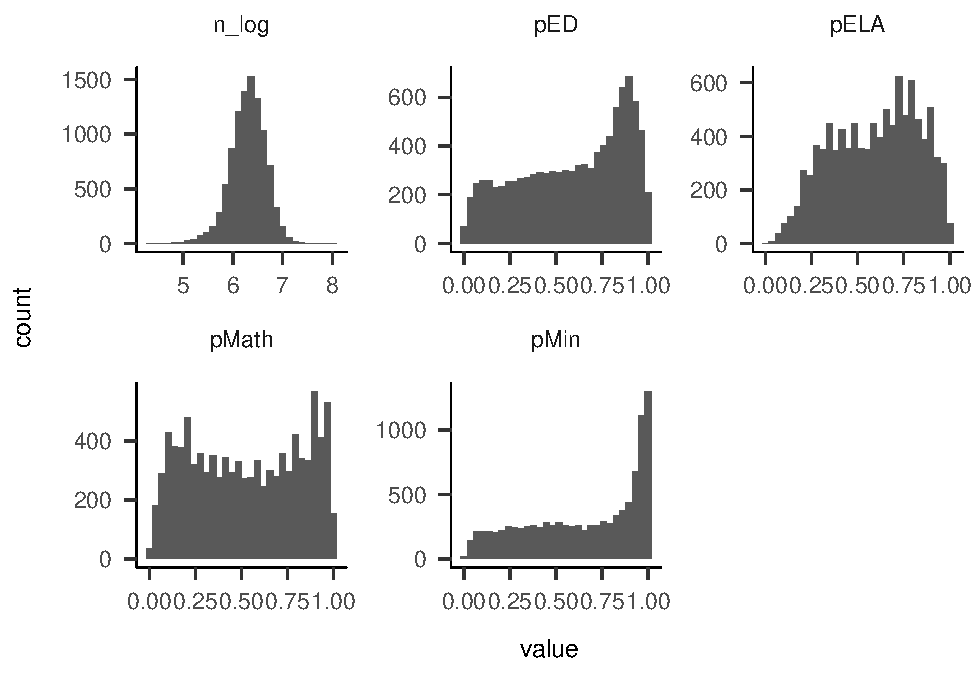
\includegraphics{GenSamp_Paper_files/figure-latex/plot-dist1-1.pdf}
\caption{\label{fig:plot-dist1}Distributions of continuous covariates. Three covariates were transformed to logs: District Size, N Students, and Student/Teachers}
\end{figure}

\hypertarget{stratification}{%
\subsection{Stratification}\label{stratification}}

We implemented stratification prior to simulation because the population is constant across iterations. Per Tipton (2013b)'s original recommendation, we use k-means clustering to partition the population into strata. This requires selecting a distance metric, choosing the number of strata, and generating the strata. All analyses were performed in R (R Core Team, 2018).

\hypertarget{cluster-analysis}{%
\subsubsection{Cluster Analysis}\label{cluster-analysis}}

We performed the cluster analysis using the \emph{cluster} package (Maechler et al., 2017). First, the \emph{daisy} function is used to compute an \(n\) by \(n\) pairwise distance matrix across all observations. This function requires two parameters: (1) the data matrix, and (2) the distance metric. The data matrix includes the full set of school level covariates used to compare schools for clustering. The distance metric summarizes the difference between a pair of sites on a set of covariates in order to maximize the similarity of all sites within a cluster. As such, the appropriate metric varies on the type of data in the matrix.

In educational research, as is the case here, data are likely to contain both continuous and categorical variables. For mixed data such as this it is appropriate to use the general similarity measure (Gower, 1971; Tipton, 2013b). This measure relies on different calculations of distance depending on the type of covariates. Let \(X_{hi}\) and \(X_{hi'}\) be the observed value of covariate \(h = {1, ..., P}\) for sites \(i\) and \(i'\) respectively, where \(i \ne i'\). Let \(d_{ii'h}\) be the distance between observed values of covariate \(X_{h}\) for site \(i\) and site \(i'\). For categorical or dummy coded variables, \(d_{ii'h} = 1\) if \(X_{hi} = X_{hi'}\) and \(d_{ii'h} = 0\) otherwise. For continuous covariates, we use the following formula:

\begin{align}
  d_{ii'h} = 1 - \frac{|X_{hi} - X_{hi'}|}{R_h}
\end{align}

where \textbar.\textbar{} indicates absolute value, and \(R_h\) is the range of observations for covariate \(X_h\). This equation restricts the range of \(d_{ii'h}\) to \([0,1]\). Finally, we calculate the general similarity between each site pair by taking the weighted average of the distances between all covariates. Let \(d^{g}_{ii'}\) be the general similarity between site \(i\) and site \(i'\).

\begin{align}
  d^{g}_{ii'} = \frac{\sum^p_{h = 1}w_{ii'h}d_{ii'h}}{\sum^p_{h = 1}w_{ii'h}}
\end{align}

where \(w_{ii'h} = 0\) if \(X_h\) is missing for either site and \(w_{ii'h} = 1\) otherwise. Setting the distance metric to \enquote{gower} in the \emph{daisy} function performs these calculations.

\hypertarget{number-of-strata}{%
\subsubsection{Number of Strata}\label{number-of-strata}}

Next we used the \emph{kmeans} function to generate clusters, which employs an optimization algorithm to classify sites into \(k\) clusters by minimizing the total within cluster variance. For each \(k\), it is recommended to run \emph{kmeans} at least 10 times, and select the clustering that results in the smallest total within-cluster sum of squares. This function also requires two parameters: (1) the distance matrix from the previous step, and (2) the number of clusters to generate (\(k\)).

Selecting an appropriate value for \(k\) is one of the most difficult problems in cluster analysis (Steinley, 2006). Tipton (2013b) states that both empirical and practical criteria should be used in selecting \(k\). A larger set of strata would result in greater homogeneity within each stratum, however it may also be more difficult to manage for recruiters. For instance, if refusal and non-response rates are fairly high, having fewer sites spread across more strata may make it difficult to adequately recruit from all strata. Resource constraints (e.g.~time, funding, recruiters) may also be a factor in the number of strata selected.

Hennig and Liao (2013) also argue that the method of selecting \(k\) should depend on the context of the clustering, framing the issue as one of obtaining an appropriate subject-matter-dependent definition rather than a statistical estimation. With these considerations in mind, we examined three criteria: (1) a generalized form of the Calinski-Harabasz index (Cali\a'nski \& Harabasz, 1974) proposed by Hennig and Liao (2013), (2) the proportion of between-cluster variance as recommended by Tipton (2013b), and (3) the practicality of sampling from fewer clusters.

Our strategy was to perform the analysis several times for each value of \(k\) and comparing all performance criteria for each set of strata generated (Figure \ref{fig:fig-k-plots}). We first calculated the Calinski-Harabasz (CH) index using the \emph{cluster.stats} function from the \emph{fpc} (Hennig ???) package. Figure \ref{fig:fig-k-plots}a displays the CH index for each \(k\) clusters generated. In this case, generating 2 clusters maximizes the CH-index. Another potential solution is at 5 clusters where there is also a local maxima.

The proportion of between-cluster variance was calculated manually. Let \(k\) be the number of strata generated where \(k = 1, 2, ..., q\) for some maximum allowable number of \(q\) strata. Let \(\sigma_{wk}^2\) be the total variability within each stratum, and \(\sigma_{bk}^2\) be the total variability between each stratum, summed across all covariates in \(X\) for each set of \(k\) strata generated. Let \(p_k\) be the proportion of variability that is between strata for each set of \(k\) strata generated be defined as follows:

\begin{align} \label{eq:pk}
  p_k = \sigma_{bk}^2/(\sigma_{wk}^2 + \sigma_{bk}^2)
\end{align}

As \(p_k\) approaches 1, most of the variation is between strata, indicating homogeneity within strata. This increases the possibility of selecting a more balanced sample. Figure \ref{fig:fig-k-plots}b plots \(p_k\) against \(k\)m allowing visual comparison of the results. The \(k\) for which the rate of change \(p_k\) slows is considered favorable. Tipton (2013b) also recommends selecting the number of clusters such that at least 80\% of the variability is between clusters, indicated by the figure as a dashed line. Given this criteria it seems that at least 7 clusters should be generated. However we also see that after a sharp initial increase, the slope of the graph begins to level out. This indicates that as we increase the number of clusters, the benefit of doing so decreases, while the difficulty of sampling from each cluster increases. In that case after 5 or 6 clusters the difficulty of sampling may not be worth such small increases in homogeneity within clusters.

Figure \ref{fig:fig-k-plots}c plots the sample size that needs to be selected from each cluster to fulfill the proportional allocation requirement such that the number of sites sampled from each cluster is proportional to the size of the cluster in the population. The dashed line indicates the ideal allocation if all clusters were of equal size. We see that the variability in cluster sizes decreases as more clusters are generated. A sensible cutoff may be determined by looking at the size of the smallest cluster. At \(k > 8\) it seems that the smallest clusters would require less than 5 sites being sampled, which may be very difficult in a practical setting. We determined that this would be the most likely criteria to be considered in the field, and ultimately decided to generate 5 clusters for this analysis.









\begin{figure}
\centering
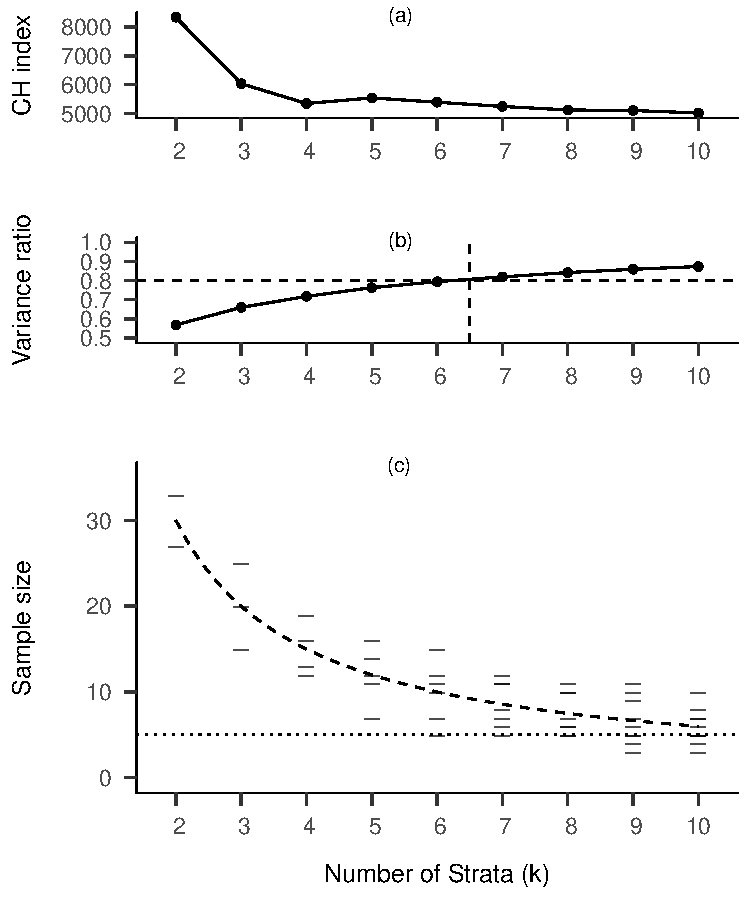
\includegraphics{GenSamp_Paper_files/figure-latex/fig-k-plots-1.pdf}
\caption{\label{fig:fig-k-plots}Plots used to determine value for \(k\). (\emph{a}) Calinski-Harabasz index - peaks indicate better fit. (\emph{b}) Ratio of between cluster sum of squares to total cluster sum of squares - horizontal line indicates cutoff of .8, vertical line indicates minimum number of clusters needed to achieve cutoff. (\emph{c}) Sampling requirements for each cluster given proportional allocation - horizontal line indicates a cluster sample size requirement of 5 schools.}
\end{figure}

\hypertarget{balanced-sampling}{%
\subsection{Balanced Sampling}\label{balanced-sampling}}

The goal of balanced sampling is to recruit in such a way that the expected value of covariate \(X_h\) across sites in stratum \(j\) is equal to the expected value of covariate \(X_h\) across all sites sampled from stratum \(j\):

\begin{align}
  E(X_ih|Z_i = 1, j) = E(X_h|j)
\end{align}

where \(Z_i = 1\) if site \(i\) is recruited into the sample and \(Z_i = 0\) otherwise. Following Tipton (2013b), we implemented balanced sampling by prioritizing the recruitment of sites based on their similarity to the \enquote{average} site in each stratum. First we identified the number of sites to be sampled from each stratum using proportional sample allocation. Each stratum contains \(N_j\) sites where \(N_1 + N_2 ... + N_k = N\). From each stratum \(j\), we calculated the number of sites to be sampled, \(n_j\), such that \(n_j = [(N_j/N)n]\), where {[}.{]} indicates that each value is rounded to the nearest integer.

Next we ranked each site within a stratum using a distance measure, with sites closer to the \enquote{center} of the strata ranked higher. We calculated the weighted Euclidean distance to the mean of each covariate:

\begin{align} \label{eq:euclid}
  d_{ij} = \sqrt{\sum^p_{h=1}w_h[X_{hij} - E(X_h|j)]^2}
\end{align}

where \(w_h\) is the weight assigned to covariate \(X_h\), \(E(X_h|j)\) is the population mean of covariate \(h\) in stratum \(j\), and \(X_{hij}\) is the value of covariate \(h\) for site \(i\) in stratum \(j\). As with generating the strata, different weights can be used such that distances depend more heavily on covariates thought to be more related to treatment effect heterogeneity. We then used the ranked list to prioritize sites for recruitment, beginning with the highest ranked sites. If a site was unavailable or refused to participate, a recruitment attempt was made with the next highest ranked site until \(n_j\) sites agreed to participate.

\hypertarget{advantages-and-limitations}{%
\subsection{Advantages and Limitations}\label{advantages-and-limitations}}

Though there are very few demonstrations of SBS in the literature, several studies outline the method's benefits (Tipton, 2013b; Tipton et al., 2016), Generally, stratified sampling methods should offer several key advantages besides better generalizability. First, the method requires that researchers document the recruitment process, carefully consider the inference population, and justify targeting specific sites. This supports transparency and enables a more careful critique of the sampling design and study inferences. Second, careful documentation also supports follow up analysis on participation behavior such as systematic differences across non-responders. Finally, SBS easily integrates with post-hoc statistical adjustment techniques. Even if balance is only partially improved at the sampling stage, coverage errors will still be reduced and less of the inference population will need to be discarded during analysis.

There are, of course, several limitations as well. SBS depends on the existence of a rich set of observed covariates related to treatment heterogeneity and sample selection for each site in the population. Most readily available extant data primarily consist of demographics and may not contain information on covariates that are more proximally related to variation in treatment effect. This can result in omitted variable bias during the cluster analysis phase (Tipton, 2013b). Additionally, SBS requires more resources to implement than a simple convenience sample. Recruiting ranked sites from multiple strata requires a coordinated effort between recruiters (Tipton, Hallberg, Hedges, \& Chan, 2017). This means that recruiters cannot work independently and must rely on a partnership with researchers implementing this method.

At least one study documents the complete implementation of SBS in a large-scale multi-site educational intervention study (Tipton \& Matlen, 2019). The authors reported that a substantial amount of time had to be dedicated to developing the sampling frame and generating optimal strata. This was compounded by the unavailability of data necessary for identifying the sampling frame (e.g.~presence of curriculum related to intervention). The recruitment effort also required a considerable amount of coordination between the researchers and the recruiters. However, the researchers were able to elicit buy-in from the recruiters, who in follow-up interviews reported that the recruitment plan and its benefits were easy to understand. Furthermore, the recruiters felt that working with strata constraints did not increase the difficulty of recruitment, though they did find that some strata were easier to recruit from than others.

\hypertarget{methods-and-models}{%
\section{Methods and Models}\label{methods-and-models}}

In this section we develop the framework for designing a study that simulates recruitment in educational research.

\hypertarget{framework-for-generalizability}{%
\subsection{Framework for Generalizability}\label{framework-for-generalizability}}

Following the framework developed by Tipton (2013b), we begin with a data set enumerating a population of \(N\) sites (schools), indexed as \(i = 1 ... N\). Each site also has a vector of observed characteristics \(X_i\) of length \(P\). The covariates are a mixture of continuous, binary, and categorical data. The goal is to select a sample of \(n\) sites such that there is balance along \(X_i\) between the sample and the population, indicating that the population is compositionally represented by the sample. We measure balance using the standardized mean difference (\(SMD\)) between the sample and population for a given covariate. \(SMD\) is calculated as

\begin{align} \label{eq:SMD}
  SMD = \frac{\bar{X}-\mu}{\sigma}
\end{align}
where \(\bar{X}\) is a vector of covariate means in the sample, \(\mu\) is the vector of covariate means in the population, and \(\sigma\) is the vector of covariate standard deviations in the population. \(SMD\) values closer to zero indicate greater balance between the sample and the population.

\hypertarget{modeling-selection-bias}{%
\subsection{Modeling Selection Bias}\label{modeling-selection-bias}}

Selection bias stems from two sources: (1) site participation behavior (self-selection) and (2) researcher sampling behavior (recruitment bias). To model the former we propose a simple participation propensity score. Let \(\pi^P_i\) represent the participation propensity score, or the probability that a site agrees to participate in an RCT if approached for recruitment. Using a simple logistic transformation we model \(\pi^P_i\) as follows:

\begin{align} \label{eq:RGM}
  log\bigg(\frac{\pi^P_i}{1 - \pi^P_i}\bigg) = \beta_0 + \boldsymbol{X_i \beta}
\end{align}
where \(\boldsymbol{X_i}\) is an \(N\) by \(P\) matrix of covariates that predict sample selection for each site, and \(\boldsymbol{\beta}\) is a vector of coefficients associated with those covariates. Participation for site \(i\) will be determined by sampling from a Bernoulli distribution with probability equal to \(\pi^P_i\).

Modeling recruitment bias is less straightforward. While self-selection is present as long as sites have the ability to choose whether or not to participate, recruitment bias depends largely on whatever strategy is used for selecting sites in the first place. It can be avoided all together by using empirical sampling techniques such as probability sampling, where the probability that a site will be invited to participate is known and can be accounted for in the outcome analysis. However, this is not often feasible in the case of large-scale MRTs. Subsets of schools are likely to be overlooked if samples are too small, or when participation rates are too low. Further, random sampling from a broad population (such as an entire country) is likely to produce samples that are geographically dispersed, creating logistic difficulties for data collection and treatment implementation. As a result, researchers often eschew probability sampling in favor of convenience sampling (Gerber \& Green, 2012; Shadish et al., 2002).

Since researchers rarely operationalize and report their process for selecting a convenience sample, the question of what drives recruitment bias, and how to model it, is left largely open-ended. As a first step, we will make an extreme assumption that the purpose of convenience sampling is to minimize effort. If we further assume that recruiters have some prior knowledge of how likely schools are to participate if approached, then we can model this selection mechanism as recruiters prioritizing schools with a higher propensity to participate.

We propose the following \enquote{low hanging fruit} approach as a preliminary model for convenience sampling. Sites are prioritized for recruitment by sequentially sampling from the population of sites using \(\pi^P_i\) as a sampling weight. Once a site is added to the list in order of priority, the probability of choosing the next site is proportional to the weights of the remaining items. In this way, sites that have higher values for \(\pi^P_i\) are more likely to be recruited earlier on.

\hypertarget{sampling-methods}{%
\subsection{Sampling Methods}\label{sampling-methods}}

Five sampling methods were compared: stratified and unstratified random sampling, stratified and unstratified convenience sampling, and stratified balanced sampling (SBS). We model the sample selection process in two stages. In the first stage, we generated indicators of \emph{potential participation}---that is, whether a school would participate in the trial \emph{if approached for recruitment}. Let \(N\) be the total number of schools in the population, and let schools be indexed by \(j = 1, ..., N\). We define \(E_j\) as a binary indicator that school \(j\) will agree to participate if contacted by recruiters, where \(E_j = 1\) if the school agrees, and \(E_j = 0\) if the school refuses. Each school was checked for approval by sampling from a Bernoulli distribution with probability equal to \(\pi^P_j\) for each school \(j\)
\begin{equation}
\label{eq:Ej}
E_j \sim B(\pi^P_j)
\end{equation}
The potential participation indicators were generated at the beginning of each iteration and were therefore common across the five sampling methods examined.

We modeled the sampling process as observing the potential participation indicator for schools in a ranked list, where the order in which schools are contacted is determined by a score \(S = S_1,...,S_N\). Let \(Z_j(S)\) be an indicator whether school \(i\) is sampled based on the score \(S\).
For the unstratified sampling methods, we determined \(Z_1(S),...,Z_N(S)\) by sorting schools according to \(S\) and selecting the first 60 schools where \(E_j = 1\).
Specifically,
\begin{equation}
\label{eq:Zj}
Z_j(S) = I\left[60 \geq \sum_{k=1}^N E_k I\left(S_k \leq S_j\right)\right]
\end{equation}
where \(I(C)\) denotes the indicator function, equal to 1 if \(C\) is true and otherwise equal to 0. Based on the sample selection indicators, we calculated the number of schools contacted as
\begin{equation}
\label{eq:R}
R(S) = \sum_{j=1}^N I(S_j \leq S_{max}),
\end{equation}
where \(S_{max} = \max \{S_1 Z_1, S_2 Z_2, ..., S_N Z_N\}\).

For the stratified sampling methods, the above process was applied within each stratum. We determined target sample sizes for each stratum based on a proportional allocation. Letting \(N_k\) denote the total number of schools in stratum \(k\), we set a target sample size of \(n_k = [60 \times N_k / N]\) for stratum \(k\), where \([x]\) is the integer nearest to \(x\).

\hypertarget{random-sampling}{%
\subsubsection{Random Sampling}\label{random-sampling}}

As previously mentioned, unstratified random sampling (URS) is typically highly impractical in the context of educational MRTs. However, URS is nonetheless interesting as a theoretically simple ideal against which to compare other sampling methods. We simulated URS sampling by ranking each school according to a random number from a uniform distribution, so that their order of recruitment was determined by the score \(S_j \sim U(0, 1)\).

In practice, methods such as cluster sampling, stratified sampling, or a combination of both would likely offer advantages over unstratified random sampling. We therefore also simulated a stratified random sample (SRS), with strata determined by the results of the cluster analysis and using a proportional allocation.

\hypertarget{convenience-sampling}{%
\subsubsection{Convenience Sampling}\label{convenience-sampling}}

We also simulated two convenience sampling methods: unstratified (UCS) and stratified convenience sampling (SCS). Here, we assumed that recruiters have some knowledge of each schools' probability of participating, if approached, and that they prioritize higher probability schools in order to minimize effort.
To operationalize unstratified convenience sampling, we assumed that schools are approached for recruitment one at a time, with their order determined by sampling without replacement, with probability proportional to participation propensity scores \(\pi^P_1,...,\pi^P_N\).
Once a school was selected and assigned a rank, the next school was selected with a probability proportional to the weights of the remaining schools. Once all ranks were assigned, schools were again approached until 60 schools agreed to be in the sample
We implemented stratified convenience sampling using the same process, but with ranks determined independently within each stratum, and using a proportional allocation across strata.

\hypertarget{balanced-sampling-1}{%
\subsubsection{Balanced Sampling}\label{balanced-sampling-1}}

SBS is unique in that rankings are directly related to school characteristics and do not change across iterations. Scores within strata were based on equation \eqref{eq:euclid} (i.e., \(S_j = d_{jk}\)), where schools closer to the \enquote{center} of the stratum are more representative of it and are therefore a higher priority. Though extremely unlikely, it is possible that several schools could be equidistant from the center of the stratum; in such cases, schools were ordered randomly.
Because Tipton (2013b) proposed balanced sampling in connection with stratification based on a cluster analysis, we only consider the stratified version, SBS.

\hypertarget{simulation-study}{%
\section{Simulation Study}\label{simulation-study}}

In this section we describe the simulation study developed to assess the generalizability of the samples selected by SBS relative to several other sampling methods, and the feasibility with which the sampling methods can be employed. A simulation study is the most convenient method for comparing multiple sampling techniques in a controlled environment. The external validity of this study largely rests on our ability to accurately model the participation propensity score. By relying on previous work and real data to inform our model, we hope to maximize how well our results represent reality. Nevertheless, given that various sampling techniques can be represented algorithmically, the relative performance of these methods should still be informative.

\hypertarget{data-generation}{%
\subsection{Data Generation}\label{data-generation}}

\hypertarget{participation-propensity-score}{%
\subsubsection{Participation Propensity Score}\label{participation-propensity-score}}

The first step was to model the participation propensity score (equation \eqref{eq:RGM}) using observed covariate values from extant school data. The set of covariates, \(X_i\), consisted of the same variables used in the cluster analysis described in Sample Frame section above. The corresponding coefficients, \(B\), were based on work by Fellers (2017) who compared 571 elementary schools that participated in IES funded studies to the full population of U.S. elementary schools. The authors reported absolute SMD between the schools that participated and the population. We standardized \(X_i\) and used reported SMDs as coefficients in equation \eqref{eq:RGM} to generated \(\pi^P_i\) values. The covariates along with the coefficient values are reported in table \ref{tab:tab-RGM-Pars}. We generate different levels of population participation rates by manipulating the intercept values. Since these rates are unknown, we selected parameters for 9 levels of participation rates.

\begin{table}[tbp]
\begin{center}
\begin{threeparttable}
\caption{\label{tab:tab-RGM-Pars}Odds ratio coefficients for Response Generating Model}
\begin{tabular}{ll}
\toprule
Variables & \multicolumn{1}{c}{log\_odds}\\
\midrule
District Size & 0.52\\
\% Black & 0.29\\
\% Hispanic & 0.40\\
\% White & -0.54\\
N Students & 0.37\\
\% ELL & 0.41\\
\% Female & -0.02\\
\% F/RL & 0.08\\
Students/Teachers & -0.10\\
Suburban & 0.01\\
Schoolwide Title I & 0.02\\
Town/Rural & -0.40\\
Urban & 0.43\\
\bottomrule
\end{tabular}
\end{threeparttable}
\end{center}
\end{table}



\hypertarget{analysis}{%
\subsection{Analysis}\label{analysis}}

\hypertarget{generalizability}{%
\subsubsection{Generalizability}\label{generalizability}}

There are several methods to quantify how generalizable a sample is to a target population. One common method is to compare the sample to the population on a range of covariates by examining SMDs as shown in equation \eqref{eq:SMD}. This method is limited as it only provides us with a measure of how close the sample means are to the population means. To have true generalizability, sample variance must also be representative of the population variance. Therefore, in addition to SMDs we also estimated the generalizability index (\(B\); Tipton, 2014).

The generalizability index is bounded between 0 and 1, with 0 indicating no overlap between the sample and the population, and 1 indicating the sample is representative of the population. First all sites in the population are divided into \(k\) bins. For bins \(j = 1,...,k\), let \(w_{pj} = N_j/N\) be the proportion of the population and \(w_{sj} = n_j/n\) be the proportion of the sample in each bin. We will calculate \(B\) as:
\begin{align}
  B = \sum^k_{j=1}\sqrt{w_{pj}w_{sj}}
\end{align}
Bins must be defined such that \(\sum{w_{pj}} = \sum{w_{sj}} = 1\). Selecting the correct number of bins is important, as too many bins will underestimate the similarity between distributions, and too few will overestimate. Tipton (2014) recommends generating equal bins of size \(h\) calculated as
\begin{align}
  h = 1.06s(N+n)^{-1/5}
\end{align}
where \(s^2\) is the pooled variance across the sample and population:
\begin{align}
  s^2 = \frac{(n - 1)s^2_s + (N + 1)s^2_p}{(N + n - 2)}
\end{align}

\hypertarget{feasibility}{%
\subsubsection{Feasibility}\label{feasibility}}

In order to assess feasibility, the total number of schools approached to achieve a full sample was tracked. The average number of refusals each sample method resulted in prior to selecting the full sample was calculated across replications. Recruiters expend a lot of resources contacting districts and schools, scheduling meetings and traveling between interested locations. A project with limited resources may not be able to afford to go through a large list of potentially uninterested sites. This measure allows us to compare the difficulty with which a full sample is recruited using each method.

\hypertarget{results}{%
\section{Results}\label{results}}

\hypertarget{generalizability-1}{%
\subsection{Generalizability}\label{generalizability-1}}

\hypertarget{b-index}{%
\subsubsection{B-Index}\label{b-index}}

Figure \ref{fig:fig-avg-Bindex} displays the average \(B\)-index for each method across participation rates. Acceptable values of \(B\) for generalizability vary depending on the size of the sample, the size of the population, and the number of covariates (Tipton, 2014). Given our design a critical value of \(B = .95\) would be needed to expect full generalizability, with lower values requiring additional statistical assistance. At population participation rates below 50\%, only SBS consistently selected highly generalizable samples. This indicates that SBS is successful at sampling schools that are unlikely to participate and therefore tend to be underrepresented by the other sampling methods, particularly when overall participation rates are low. Stratified random sampling consistently outperformed simple random sampling across all participation rates, though only slightly.

We also found several trends that were unexpected. At 50\% and beyond, SBS performance slowly degrades, while other methods maintain a steady increase. We expected a constant positive relationship between the population participation rate and the performance of all methods. Furthermore, at low response rates unstratified convenience sampling seemed to perform better than stratified convenience sampling. This seems counter-intuitive, as survey literature suggests that stratified samples are more representative. Because the B-index is an overall measure of generalizabilty across many covariates, it is difficult to untangle why these methods preformed as they did. The next section will examine the models' performance for each covariate.



\begin{figure}
\centering
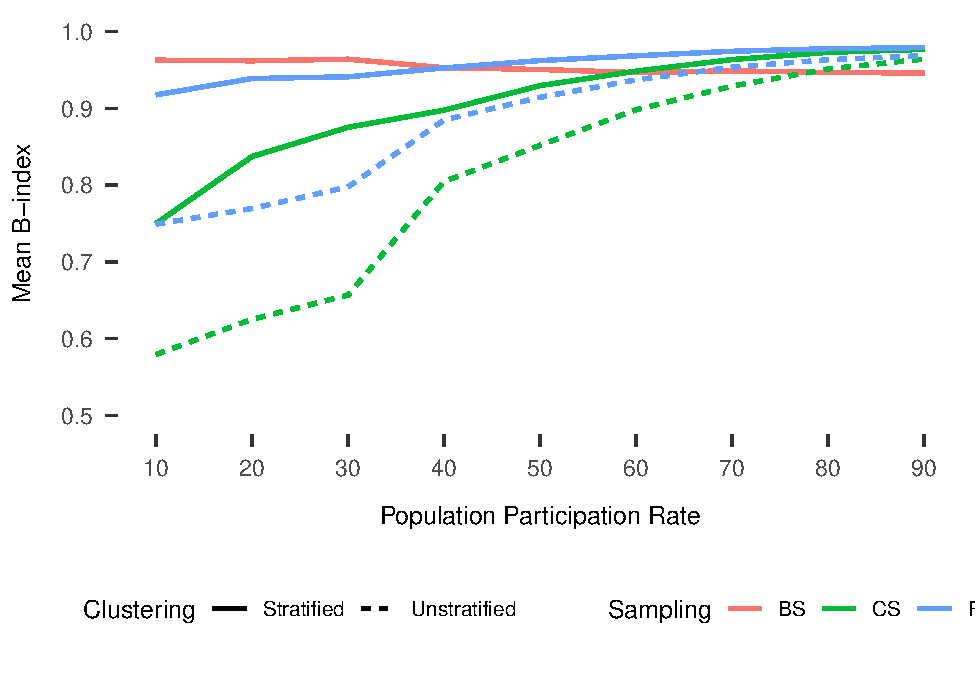
\includegraphics{GenSamp_Paper_files/figure-latex/fig-avg-Bindex-1.pdf}
\caption{\label{fig:fig-avg-Bindex}Average \(B\)-index for varying participation rates, by sampling method. Horizontal dotted line represented index of .95 indicating a high level of generalizability.}
\end{figure}

\hypertarget{standardized-mean-differences}{%
\subsubsection{Standardized Mean Differences}\label{standardized-mean-differences}}

One potential explanation for why stratification may under-perform in certain circumstances is if the strata do not explain any variance in a covariate that is related to participation. To examine this we calculated the ICC for each covariate across strata and compared it to the log-odds coefficients associated with that covariate in the participation response model. Table \ref{tab:tab-ICC-Pars} displays these values. Examining these along with SMDs uncovered several patterns which are summarized in figure \ref{fig:fig-ICCvsCoef}.

\begin{table}[tbp]
\begin{center}
\begin{threeparttable}
\caption{\label{tab:tab-ICC-Pars}Odds ratio coefficients and strata ICC}
\begin{tabular}{llll}
\toprule
Variables & ICC & Absolute Log Odds & Quality\\
\midrule
Schoolwide Title I & 0.94 & 0.02 & Good1\\
\% F/RL & 0.76 & 0.08 & Good1\\
Urban & 0.91 & 0.43 & Good1\\
\% White & 0.67 & 0.54 & Good1\\
\% Hispanic & 0.66 & 0.40 & Good1\\
\% ELL & 0.54 & 0.41 & Good1\\
Suburban & 0.58 & 0.01 & Good2\\
Town/Rural & 0.27 & 0.40 & Good2\\
District Size & 0.12 & 0.52 & Good2\\
\% Female & 0.00 & 0.02 & Neutral\\
Students/Teachers & 0.10 & 0.10 & Neutral\\
N Students & 0.06 & 0.37 & Bad\\
\% Black & 0.06 & 0.29 & Bad\\
\bottomrule
\end{tabular}
\end{threeparttable}
\end{center}
\end{table}



\begin{figure}
\centering
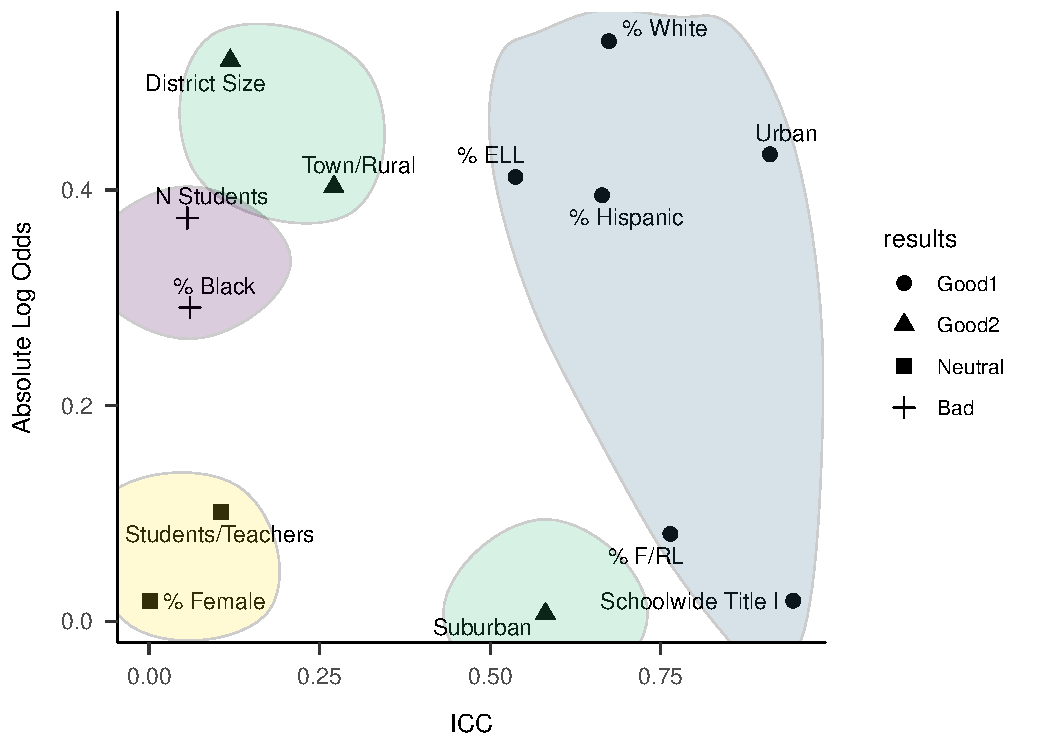
\includegraphics{GenSamp_Paper_files/figure-latex/fig-ICCvsCoef-1.pdf}
\caption{\label{fig:fig-ICCvsCoef}ICC Values vs absolute log odds. Shaded areas illustrate potential patterns in generalizability measured by SMDs.}
\end{figure}

First, figure \ref{fig:fig-SMD-by-Var-good1} displays six covariates where both ICC values and response generating model parameters were high. For these covariates, SBS performed as well as or better than all stratified methods, and all stratified methods performed better than their unstratified counterparts. Figure \ref{fig:fig-SMD-by-Var-neutral} displays two covariates where both ICC values and response generating model parameters were low. SBS seemed to perform slightly better than all other methods, however all methods performed well across all population participation rates.



\begin{figure}
\centering
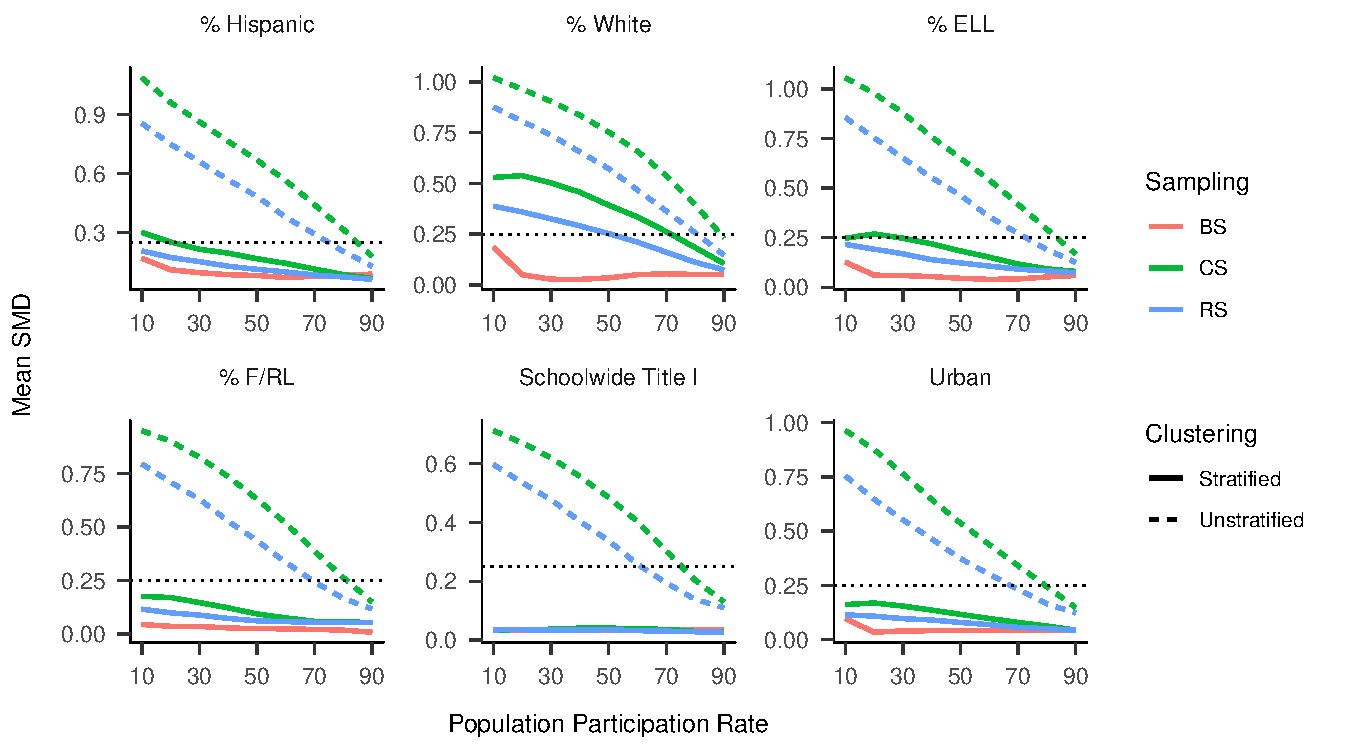
\includegraphics{GenSamp_Paper_files/figure-latex/fig-SMD-by-Var-good1-1.pdf}
\caption{\label{fig:fig-SMD-by-Var-good1}Good balance for stratified methods. Dotted horizontal line indicates a .25 cutoff.}
\end{figure}



\begin{figure}
\centering
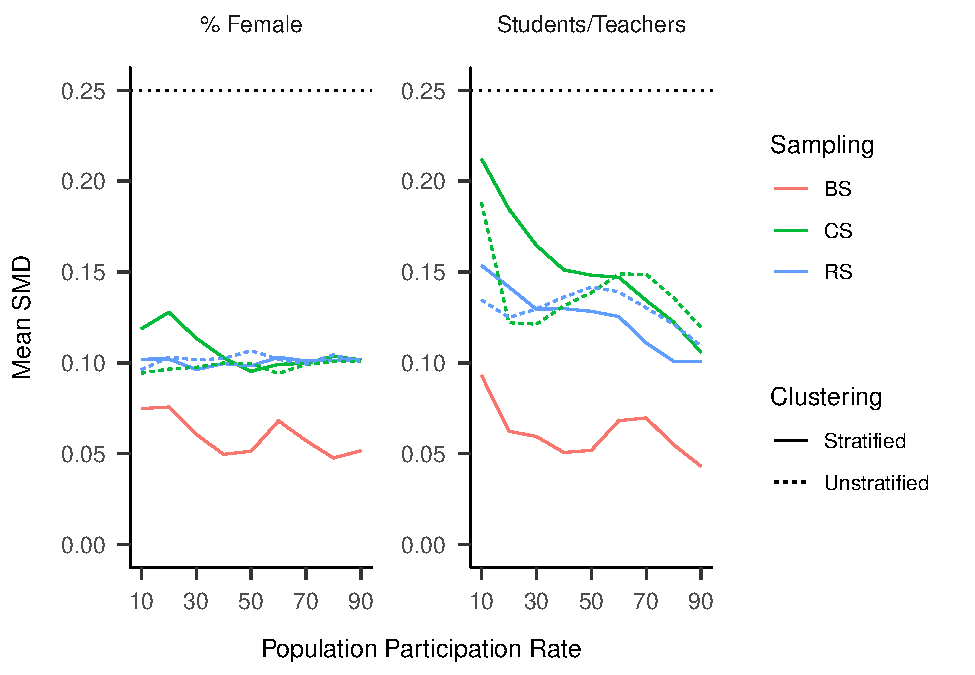
\includegraphics{GenSamp_Paper_files/figure-latex/fig-SMD-by-Var-neutral-1.pdf}
\caption{\label{fig:fig-SMD-by-Var-neutral}All methods performed well. Dotted horizontal line indicates a .25 cutoff.}
\end{figure}

Figure \ref{fig:fig-SMD-by-Var-good2} reports the first set of unexpected results. For three covariates, stratified random sampling and stratified convenience sampling outperform their unstratified counterparts. However, for district size, SBS seems to perform more poorly as the population participation rate increases. For suburban and town/rural indicators, this is the only time where SBS performs poorly using the SMD criteria, but only in lower population participation rates. Examining table \ref{tab:tab-ICC-Pars} suggests that this pattern emerges when ICC values are moderate and response generating model parameters either high or low.



\begin{figure}
\centering
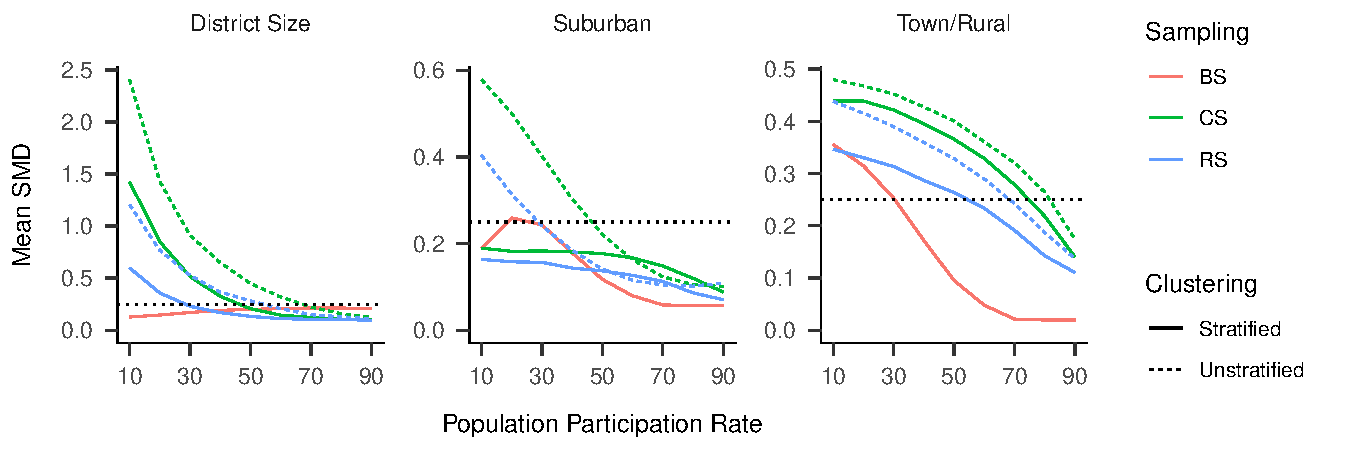
\includegraphics{GenSamp_Paper_files/figure-latex/fig-SMD-by-Var-good2-1.pdf}
\caption{\label{fig:fig-SMD-by-Var-good2}Good balance for stratified methods. Dotted horizontal line indicates a .25 cutoff.}
\end{figure}

Finally, figure \ref{fig:fig-SMD-by-Var-bad} reports the second set of unexpected results. For two covariates, SBS seems to perform well. However, stratified random sampling and stratified convenience sampling perform worse than their unstratified counterparts. For \% black SBS performance also seems to slightly degrade as population participation rates increase. Examining table \ref{fig:tab-ICC-Pars} suggests that this pattern emerges when ICC values close to zero and response generating model parameters are moderate or higher



\begin{figure}
\centering
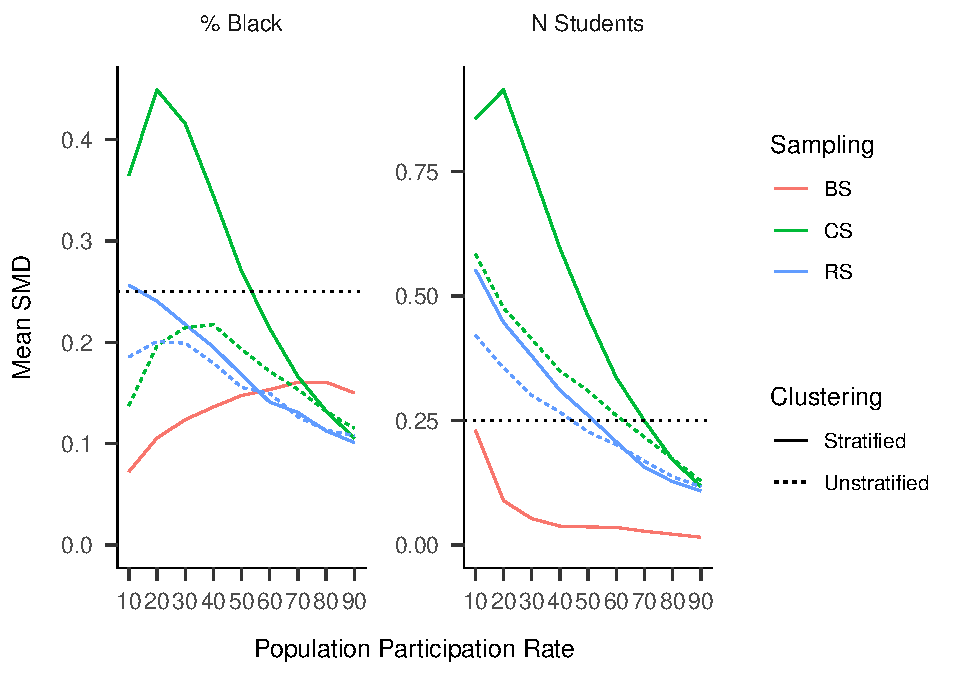
\includegraphics{GenSamp_Paper_files/figure-latex/fig-SMD-by-Var-bad-1.pdf}
\caption{\label{fig:fig-SMD-by-Var-bad}Poor balance for stratified methods. Dotted horizontal line indicates a .25 cutoff.}
\end{figure}

\hypertarget{feasibility-1}{%
\subsection{Feasibility}\label{feasibility-1}}

\hypertarget{recruitment-attempts}{%
\subsubsection{Recruitment Attempts}\label{recruitment-attempts}}

Figure \ref{fig:fig-responses} reports the sampling statistics for each method across population participation rates. Differences between sampling methods were substantial at lower participation rates. As participation rates increased, the differences decreased exponentially and became negligent. It's important to note that the magnitudes of these results are quite extreme. This is likely due to some misspecification on the part of the simulation either in the response generating model parameters or the population participation rates. Rather than looking at the raw values, a more meaningful interpretation would be to compare the performance of the models relative to each other.

Overall, UCS required the least \enquote{effort} to recruit a full sample, followed by URS and SCS, SRS, and finally SBS. Figure \ref{fig:fig-comp} plots proportional relative difficult of the models to each other. At a population response rate of 10\%, SBS compared to UCS required approximately 22 times the number of schools to be contacted. Relative to URS, SBS required about 7 times as many recruitment attempts. The 10\% response rate is likely a severe underestimate of the true population response rate and should therefore be read interpreted as an absolute worst case.



\begin{figure}
\centering
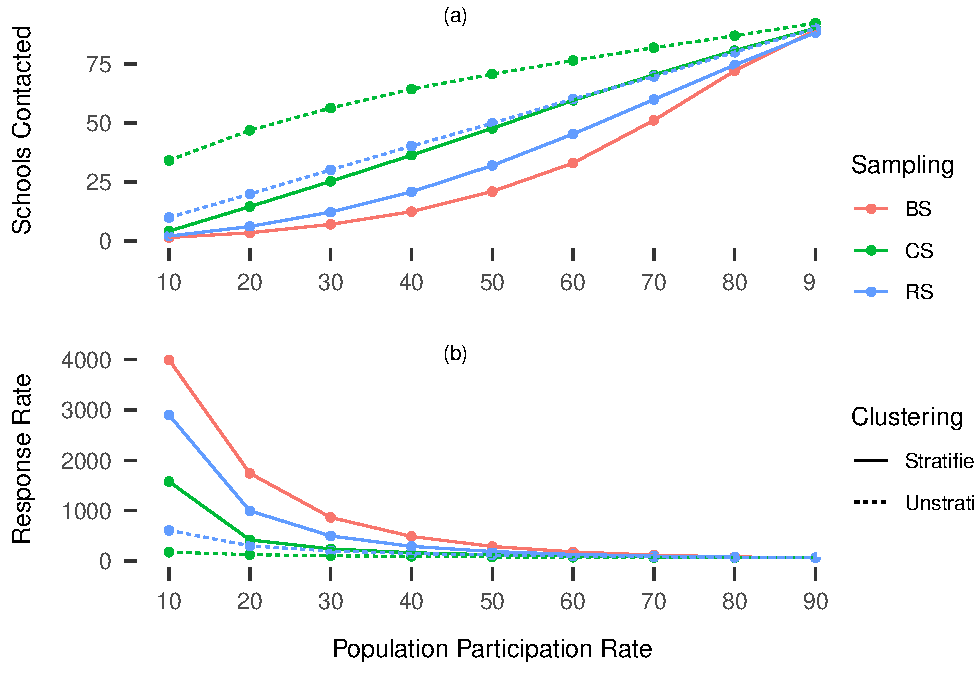
\includegraphics{GenSamp_Paper_files/figure-latex/fig-responses-1.pdf}
\caption{\label{fig:fig-responses}Sampling statistics. The top plot shows the total number of units contacted to achieve a full sample of 60 schools. The bottom plot shows the percent of schools that agreed to participate when recruited.}
\end{figure}



\begin{figure}
\centering
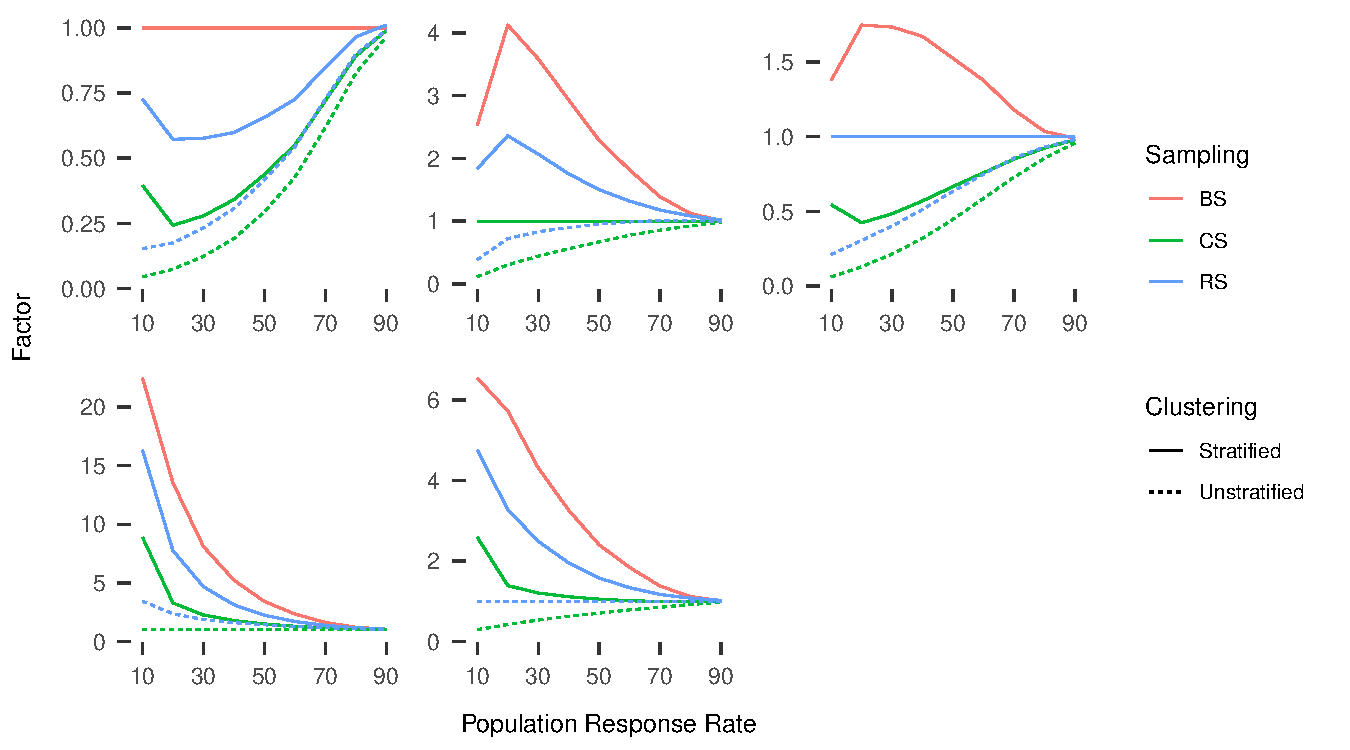
\includegraphics{GenSamp_Paper_files/figure-latex/fig-comp-1.pdf}
\caption{\label{fig:fig-comp}Proportionate comparisons of difficulties between models. The straight horizontal line is the focus of comparison in each panel.}
\end{figure}





\hypertarget{gini-plot}{%
\subsubsection{Gini Plot}\label{gini-plot}}

We calculated the Gini coefficient for each sampling method to examine the equality of sampling probabilities across methods. Figure Gini coefficient across participation response rates for each sampling method. A coefficient of 1 indicates major inequality in sampling probability. displays these for each sampling method across population participation rates. A coefficient of 1 indicates substantial sampling inequality. In the context of the simulation, this indicates that across iterations, only a small subset of the population was ever actually sampled. Several trends emerged in this analysis. As population participation rates increased, inequality increased when using SBS, and decreased when using any other method. These four other methods also performed consistently relative to one another, with SRS resulting in the least amount of sampling inequality, followed by URS, SCS and UCS. One exception is when the population response rate was set to 90\%, where the unstratified and stratified versions of RS and CS seemed to perform equally. This finding suggests that stratifying the population results in a larger potential sampling pool. However, the method for selecting units from within each stratum may ultimately nullify this difference.



\begin{figure}
\centering
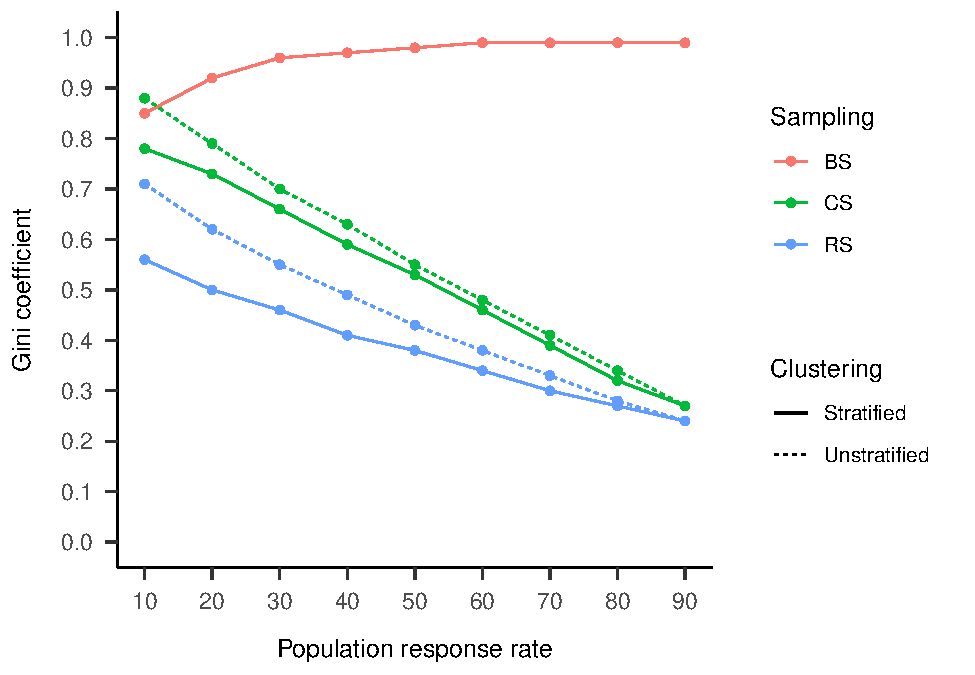
\includegraphics{GenSamp_Paper_files/figure-latex/fig-gini-1.pdf}
\caption{\label{fig:fig-gini}Gini coefficient across participation response rates for each sampling method. A coefficient of 1 indicates major inequality in sampling probability.}
\end{figure}



\begin{sidewaysfigure}
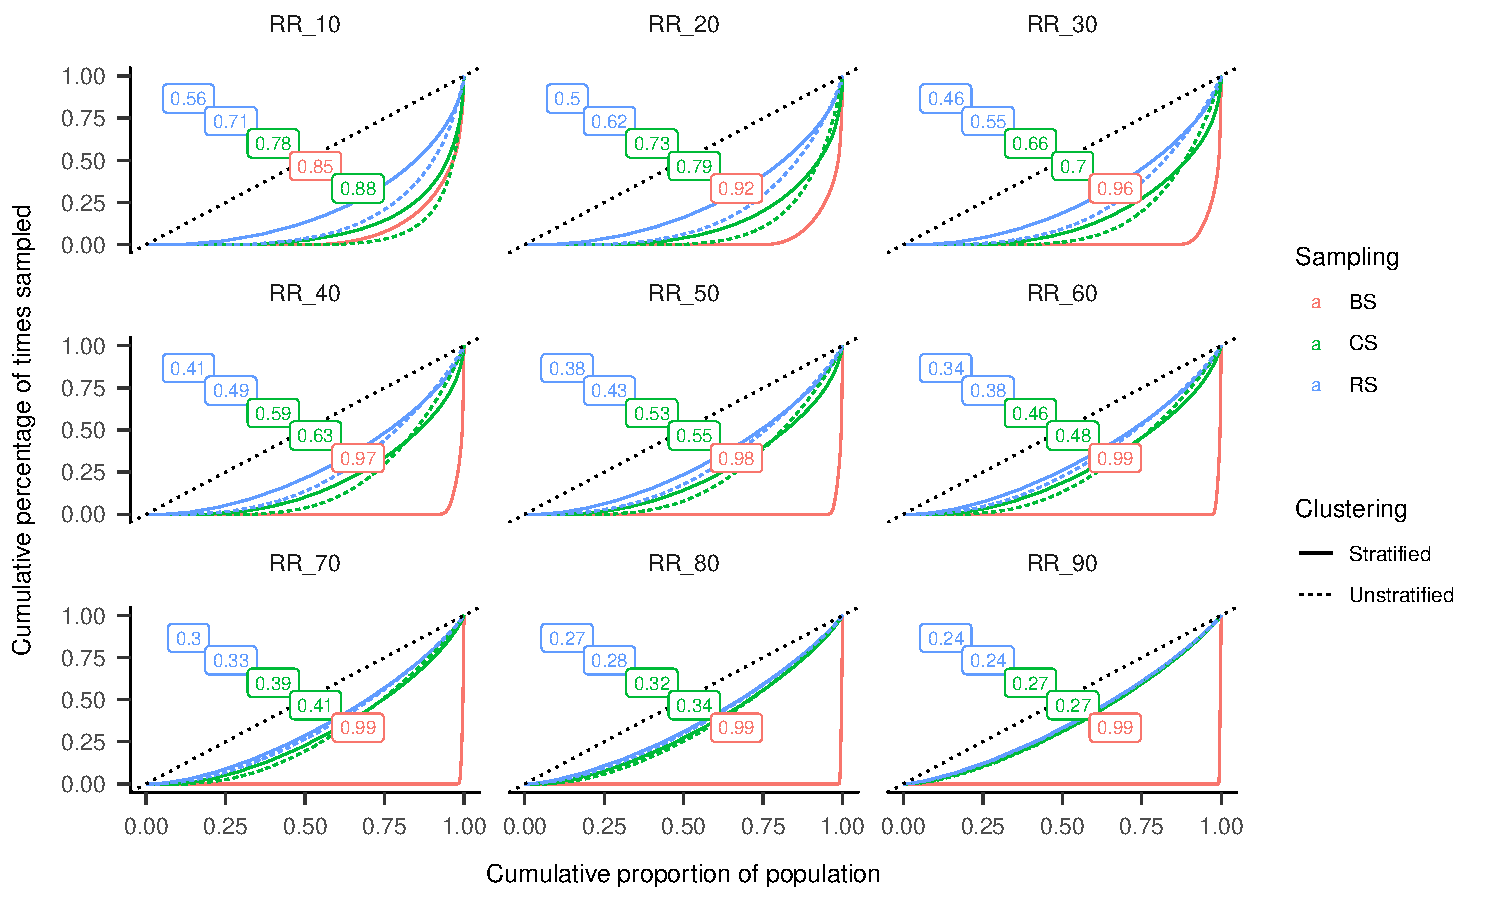
\includegraphics{GenSamp_Paper_files/figure-latex/fig-gini-curve-1} \caption{Gini plot and coefficient representing the inequality of school sampling across sampling methods and population response rates.}\label{fig:fig-gini-curve}
\end{sidewaysfigure}

\hypertarget{summary-of-trends}{%
\subsection{Summary of Trends}\label{summary-of-trends}}

In terms of selecting a generalizable sample, SBS resulted in a considerable improvement compared to UCS. However, given the difficulty with which those samples are recruited, SBS is unlikely to be fully implemented in the ideal form. Instead, SCS may be a reasonable compromise. Our findings indicate that any sampling method is greatly improved by first stratifying the population. We show that, in certain cases, performing a convenience sample within strata (SCS) is comparable to simple random sampling (URS) both in terms of generalizability and feasibility.

An exception to this seems to be driven largely by the accuracy of the clustering method with respect to the response model. For instance, in Figure \ref{fig:fig-SMD-by-Var-bad} we see that all methods of sampling result in balance on percentage of Black students, except for stratified convenience sampling. This is likely a result of the covariate having a strong relationship with participation, but not being weighed enough in the cluster analysis during stratification. Figure \ref{fig:fig-ICCvsCoef} displays the calculated intraclass correlation coefficient (ICC) for each covariate along the strata, and the coefficient for each covariate in the response generating model. For covariates where one value (ICC or coefficient) is high, while the other is low, stratified sampling techniques resulted in poor balance.

\hypertarget{discussion}{%
\section{Discussion}\label{discussion}}

The main goal of this study was to develop a framework for exploring the performance of sampling methods within the educational context. Prior to our work there has been no precedent for algorithmically modeling how researchers may select convenience sample of schools. Similarly we found no prior work attempting to model whether or not schools would participate in a study if recruited. The methods we proposed for modeling these behaviors can easily be extended to more complex and realistic specifications and adapted to any relevant population frame.

A secondary goal was to use this framework in a demonstration of several sampling methods and their relative performance in terms of generalizability and feasibility. From this work we have drawn several conclusions. Stratified balanced sampling as proposed by Tipton (2013b) has the potential to greatly increase the generalizability of samples selected for MRTs. However, this method is not without limitations. Within our simulation, strict adherence came at a great cost in terms of sheer number of schools that needed to be contacted. In practice this could mean that many more resources must be allocated to recruitment if this method is to be implemented.

We found that improper specification during the cluster analysis stage may also attenuate the generalizability of the sample. Covariates that were improperly prioritized when generating the strata wound up being poorly represented in the final samples. This can potentially nullify the investment of resources into SBS. Finally, while the balanced sampling approach does result in greater generalizability, it also appears to limit the actual pool of potential participants. Particularly in larger population response rates, the same subset of schools were likely to be recruited across iterations.

One potential compromise is generate strata, and to implement convenience sampling within strata as demonstrated by SCS. This often resulted in better balance on individual covariates than simple random sampling, which is touted as the generalizability gold standard. Beyond generalizability, stratifying in this manner offers the additional advantage of transparency by forcing the researcher to make sampling decisions in the study design phase, and to keep track of sampling decisions as recruitment is implemented.

\hypertarget{limitations}{%
\subsection{Limitations}\label{limitations}}

The sampling methods we developed made several assumptions which represent limitations of the findings from the simulation study. First, in modeling convenience sampling, we assumed that recruiters always prioritize schools that are most likely to participate. In truth, many other factors play a role such as proximity of sample sites to the researcher and to each other, existing relationships between the recruiters and the sample sites, and other researcher assumptions about the sample site's characteristics. This limits how well our results reflect the performance of models in reality.

Another implication of this assumption is that recruiters have approximate knowledge of how likely a sampled site is to participate. Though researchers may speculate about sites that are more willing to participate (schools in larger urban districts) and prioritize recruiting such sites, it is not likely that they would estimate willingness as well as we have simulated. Given this, it is possible that the \enquote{feasibility} of the convenience methods is over-stated, and that the degree of generalizability for some covariates is under-stated.

It is worth refining and exploring additional methods for modeling convenience sampling. The algorithms used in these methods can easily be tuned to include additional weights for prioritizing school recruitment. For instance, location data is readily available and can therefore be used to model some relationship between prioritizing a school and it's proximity to a researcher. Further work here can provide more realistic and practical estimations of feasibility and generalizabilty, and can provide researchers with a tool for evaluation sampling methods given their unique circumstances during the study design phase.

The second set of assumptions deals with the speculative nature of our participation model. The decision of whether a school participates in such a study is multi-leveled. Generally, districts serve as gatekeepers, requiring submission and approval of research requests prior to recruitment. If the request is denied, no schools within the district may be recruited. If approved, researchers may work with a district wide school coordinator, or may have to contact schools individually. In both cases, the ultimate decision then rest with administrators, school research coordinators, or the teachers themselves.

Additionally, the parameters in our response generating model are based on values from a study that examined the difference between schools participating in large-scale RCTs and the overall population of schools. However, these RCTs themselves typically rely on some form of convenience sampling. In that sense our parameters reflect participation rates of schools that are likely to participate in RCTs, rather than the full population of schools.

Despite this limitations, we believe that our findings reasonably represent the relative performance of the various sampling methods we tested in the context of educational research. However, this calls for a more exhaustive look at what drives school participation in the population. Disentangling participation bias from sampling bias requires researchers to implement probability based sampling or to be more transparent about their sampling practices. In this manner, we can begin identifying schools that are consistently and systematically under represented and developing strategies to target such schools, thus increasing the inclusivity of studies that strive for truly representative population level inferences.

\hypertarget{future-directions}{%
\subsection{Future Directions}\label{future-directions}}

Our work in this study has exposed several avenues of research that worth exploring within this context. First, additional work needs to be done exploring how best to optimize the cluster analysis. We have shown that the extent to which balance is achieved on a given covariate is related to how much that covariate drives strata generation and school participation. If some covariates are known to have greater influence on school participation, they may be wroth weighing more heavily in generating the strata. Furthermore, the relationship between number of clusters generated, generalizability, and feasibility is unknown. It is expected that more clusters would increase generalizability, but also make recruitment more difficult. Knowing these relationships could help drive decision making as the sampling model is being specified.

Further work also needs to examine the impact of these sampling methods on actual treatment effect estimates. In this study, our goal was only to select a generalizable sample. However, treatment heterogeneity is the ultimate culprit in the generalizability problem. Our results can be extrapolated to effect estimation only to the extent that there is complete overlap between covariates that predict sample selection and treatment heterogeneity. This is unlikely to be the case in reality, which further complicates the specification of the cluster analysis. How should covariates be weighed relative to each other depending on whether they predict participation, differences in treatment effects, or some combination of both? To address this our work must be extended to study the relationship between sampling methods and bias in treatment effect estimation.

Large scale MRTs are expensive to implement, and resource allocation for such a study is a difficult process. Researchers who wish to invest in robust recruitment strategies to amplify the impact and relevance of of their work should be better equipped to anticipate the costs and benefits of various sampling strategies. We hope that by showing the relative performance of these sampling methods, and by demonstrating the implementation of stratified sampling, we have contributed to future researchers being better informed in making these decisions.

\hypertarget{references}{%
\section{References}\label{references}}

\begingroup
\setlength{\parindent}{-0.5in}
\setlength{\leftskip}{0.5in}

\hypertarget{refs}{}
\leavevmode\hypertarget{ref-calinskiDendriteMethodCluster1974}{}%
Cali\a'nski, T., \& Harabasz, J. (1974). A dendrite method for cluster analysis. \emph{Communications in Statistics}, \emph{3}(1), 1--27. doi:\href{https://doi.org/10.1080/03610927408827101}{10.1080/03610927408827101}

\leavevmode\hypertarget{ref-fellersDevelopingApproachDetermine2017}{}%
Fellers, L. (2017). \emph{Developing an approach to determine generalizability: A review of efficacy and effectiveness trials funded by the Institute of Education Sciences} (Ph.D.). Columbia University, United States -- New York. Retrieved from \url{https://search.proquest.com/docview/1865595768/abstract/40FD82F4A0C24535PQ/1}

\leavevmode\hypertarget{ref-gerberFieldExperimentsDesign2012}{}%
Gerber, A. S., \& Green, D. P. (2012). \emph{Field experiments: Design, analysis, and interpretation} (1st ed.). New York: W. W. Norton.

\leavevmode\hypertarget{ref-gowerGeneralCoefficientSimilarity1971}{}%
Gower, J. C. (1971). A General Coefficient of Similarity and Some of Its Properties. \emph{Biometrics}, \emph{27}(4), 857--871. doi:\href{https://doi.org/10.2307/2528823}{10.2307/2528823}

\leavevmode\hypertarget{ref-grovesSurveyMethodology2004}{}%
Groves, R. M. (Ed.). (2004). \emph{Survey methodology}. Hoboken, N.J: Wiley-Interscience.

\leavevmode\hypertarget{ref-hennigHowFindAppropriate2013}{}%
Hennig, C., \& Liao, T. F. (2013). How to find an appropriate clustering for mixed-type variables with application to socio-economic stratification: How to Find an Appropriate Clustering. \emph{Journal of the Royal Statistical Society: Series C (Applied Statistics)}, \emph{62}(3), 309--369. doi:\href{https://doi.org/10.1111/j.1467-9876.2012.01066.x}{10.1111/j.1467-9876.2012.01066.x}

\leavevmode\hypertarget{ref-kernAssessingMethodsGeneralizing2016}{}%
Kern, H. L., Stuart, E. A., Hill, J., \& Green, D. P. (2016). Assessing Methods for Generalizing Experimental Impact Estimates to Target Populations. \emph{Journal of Research on Educational Effectiveness}, \emph{9}(1), 103--127. doi:\href{https://doi.org/10.1080/19345747.2015.1060282}{10.1080/19345747.2015.1060282}

\leavevmode\hypertarget{ref-olsenExternalValidityPolicy2013}{}%
Olsen, R. B., Orr, L. L., Bell, S. H., \& Stuart, E. A. (2013). External Validity in Policy Evaluations That Choose Sites Purposively. \emph{Journal of Policy Analysis and Management}, \emph{32}(1), 107--121. doi:\href{https://doi.org/10.1002/pam.21660}{10.1002/pam.21660}

\leavevmode\hypertarget{ref-omuircheartaighGeneralizingUnrepresentativeExperiments2014}{}%
O'Muircheartaigh, C., \& Hedges, L. V. (2014). Generalizing from unrepresentative experiments: A stratified propensity score approach. \emph{Journal of the Royal Statistical Society: Series C (Applied Statistics)}, \emph{63}(2), 195--210. doi:\href{https://doi.org/10.1111/rssc.12037}{10.1111/rssc.12037}

\leavevmode\hypertarget{ref-raudenbushStatisticalPowerOptimal2000}{}%
Raudenbush, S. W., \& Liu, X. (2000). Statistical power and optimal design for multisite randomized trials. \emph{Psychological Methods}, \emph{5}(2), 199--213. doi:\href{https://doi.org/10.1037//1082-989X.5.2.199}{10.1037//1082-989X.5.2.199}

\leavevmode\hypertarget{ref-shadishExperimentalQuasiexperimentalDesigns2002}{}%
Shadish, W. R., Cook, T. D., \& Campbell, D. T. (2002). \emph{Experimental and quasi-experimental designs for generalized causal inference}. Boston, MA, US: Houghton, Mifflin and Company.

\leavevmode\hypertarget{ref-steinleyKmeansClusteringHalfcentury2006}{}%
Steinley, D. (2006). K-means clustering: A half-century synthesis. \emph{British Journal of Mathematical and Statistical Psychology}, \emph{59}(1), 1--34. doi:\href{https://doi.org/10.1348/000711005X48266}{10.1348/000711005X48266}

\leavevmode\hypertarget{ref-stuartCharacteristicsSchoolDistricts2017}{}%
Stuart, E. A., Bell, S. H., Ebnesajjad, C., Olsen, R. B., \& Orr, L. L. (2017). Characteristics of School Districts That Participate in Rigorous National Educational Evaluations. \emph{Journal of Research on Educational Effectiveness}, \emph{10}(1), 168--206. doi:\href{https://doi.org/10.1080/19345747.2016.1205160}{10.1080/19345747.2016.1205160}

\leavevmode\hypertarget{ref-stuartUsePropensityScores2011}{}%
Stuart, E. A., Cole, S. R., Bradshaw, C. P., \& Leaf, P. J. (2011). The use of propensity scores to assess the generalizability of results from randomized trials: Use of Propensity Scores to Assess Generalizability. \emph{Journal of the Royal Statistical Society: Series A (Statistics in Society)}, \emph{174}(2), 369--386. doi:\href{https://doi.org/10.1111/j.1467-985X.2010.00673.x}{10.1111/j.1467-985X.2010.00673.x}

\leavevmode\hypertarget{ref-tiptonImprovingGeneralizationsExperiments2013}{}%
Tipton, E. (2013a). Improving Generalizations From Experiments Using Propensity Score Subclassification: Assumptions, Properties, and Contexts. \emph{Journal of Educational and Behavioral Statistics}, \emph{38}(3), 239--266. Retrieved from \url{https://www.jstor.org/stable/41999424}

\leavevmode\hypertarget{ref-tiptonStratifiedSamplingUsing2013}{}%
Tipton, E. (2013b). Stratified Sampling Using Cluster Analysis: A Sample Selection Strategy for Improved Generalizations From Experiments. \emph{Evaluation Review}, \emph{37}(2), 109--139. doi:\href{https://doi.org/10.1177/0193841X13516324}{10.1177/0193841X13516324}

\leavevmode\hypertarget{ref-tiptonHowGeneralizableYour2014}{}%
Tipton, E. (2014). How Generalizable Is Your Experiment? An Index for Comparing Experimental Samples and Populations. \emph{Journal of Educational and Behavioral Statistics}, \emph{39}(6), 478--501.

\leavevmode\hypertarget{ref-tiptonSiteSelectionExperiments2016}{}%
Tipton, E., Fellers, L., Caverly, S., Vaden-Kiernan, M., Borman, G., Sullivan, K., \& de Castilla, V. R. (2016). Site Selection in Experiments: An Assessment of Site Recruitment and Generalizability in Two Scale-up Studies. \emph{Journal of Research on Educational Effectiveness}, \emph{9}(sup1), 209--228. doi:\href{https://doi.org/10.1080/19345747.2015.1105895}{10.1080/19345747.2015.1105895}

\leavevmode\hypertarget{ref-tiptonImplicationsSmallSamples2017}{}%
Tipton, E., Hallberg, K., Hedges, L. V., \& Chan, W. (2017). Implications of Small Samples for Generalization: Adjustments and Rules of Thumb. \emph{Evaluation Review}, \emph{41}(5), 472--505. doi:\href{https://doi.org/10.1177/0193841X16655665}{10.1177/0193841X16655665}

\leavevmode\hypertarget{ref-tiptonImprovedGeneralizabilityImproved2019}{}%
Tipton, E., \& Matlen, B. J. (2019). Improved Generalizability Through Improved Recruitment: Lessons Learned From a Large-Scale Randomized Trial. \emph{American Journal of Evaluation}, \emph{40}(3), 414--430. doi:\href{https://doi.org/10.1177/1098214018810519}{10.1177/1098214018810519}

\endgroup


\end{document}
